%!TEX root = /Users/dbreuer/Documents/Work/_FH/_Master/master_thesis/Main/Master Thesis.tex

\chapter{Szenario} % (fold)
\label{cha:szenario}

  Wie bereits im vorangegangen Kapitel erwähnt, liegt dem COSIMA-Projekt ein dediziertes Vorgehensmodell zu Grunde, dass speziell für dieses Projekt entwickelt wurde~\citep[S. 7]{bericht}. Die schematische Darstellung dieses Modell findet sich in Abbildung~\ref{fig:vorgehensmodell}. Im Folgenden sind die Kernpunkte dieses Vorgehens zusammengefasst:

  \begin{figure}[!ht]
    \centering
      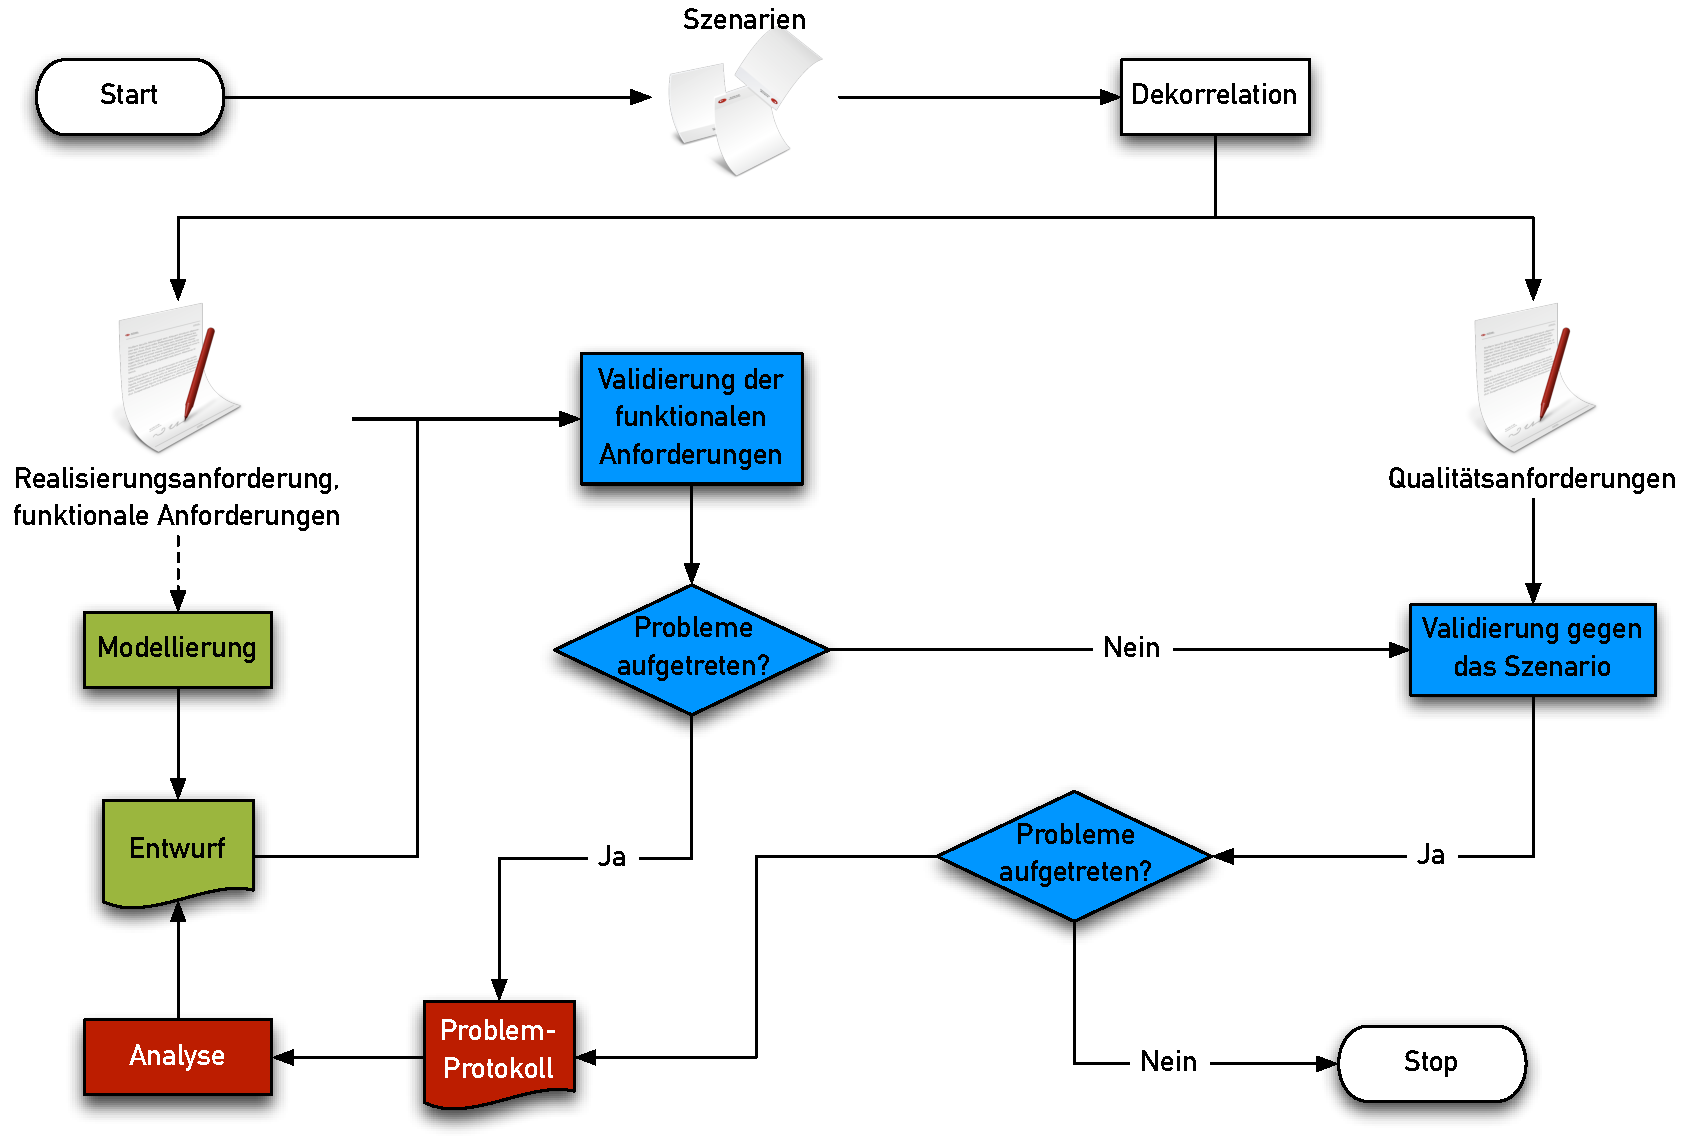
\includegraphics[width=.9\textwidth]{images/Vorgehensmodell}
    \caption{Schematische Darstellung des Vorgehensmodell hinter dem COSIMA-Projekt (nach~\citep{bericht})}
    \label{fig:vorgehensmodell}
  \end{figure}

  \begin{description}
    \item[Iterativ] Ein Iteratives Vorgehen bei der Entwicklung von Software ist ein etabliertes Verfahren, um der Unvollständigkeit der Anforderungsermittlung gerecht zu werden~\citep{brooks1987nsb,basili2005iea,boehm1986sm,kruchten2003rup}. Da auch im COSIMA-Projekt nicht zu erwarten war, dass alle relevanten Anforderungen von Anfang offensichtlich sind, wurde sich in diesem Kontext ein iterativer Prozess gewählt.
    \item[Szenario-basiert] Die Verwendung von Szenarien ist in vielen Bereichen der Softwareentwicklung\footnote{Neben der Architekturentwicklung~\citep{software_architecture_in_practice,scenario_based_software_architecture_evaluation_methods} und der Anforderungsermittlung~\citep{weidenhaupt1998sus}, etwa im Bereich der Mensch-Computer-Interaktion~\cite{five_reasons_for_scenario_based_design}.} ein anerkanntes Verfahren um Anforderungen und Qualitätsmerkmale von Software konkret zu formulieren.
    \item[Top-Down] Es werden zuerst abstrakte Szenarien definiert, die zum einen sehr informell, zum anderen sowohl funktionale, wie auch nicht-funktionale Anforderungen in sich vereinen\footnote{Nach ~\citep[S. 42f]{weidenhaupt1998ssd} ist dieses Vorgehen auch bei anderen Szenario-basierten Modellen durchaus üblich.}. Im Zuge der Iterationen werden diese Szenarien immer detaillierter und formeller. Die Architektur entwickelt sich entsprechend ebenso weiter. Daher kann man hier von einem \emph{top-down} Vorgehen sprechen.
  \end{description}
  
  Ein elementarer Bestandteil dieses Vorgehenmodells ist also die Verwendung von Szenarien. Da diese Arbeit erstens in das Umfeld des COSIMA-Projekts einzuordnen ist und Szenarien eine anerkannte Methodik darstellen, werden sie auch in dieser Arbeit dazu verwendet die bisherige Architektur zu validieren. Im Folgenden Abschnitt wird der Begriff des Szenario genauer definiert und eingeordnet. Bevor dann das eigentliche Szenario dargestellt wird, findet noch eine Abgrenzung zu Szenarien statt, wie sie in der Literatur beschriebenen szenario-basierten Methodiken Verwendung finden.
  
\section{Definition: Szenario} % (fold)
\label{sec:definition_szenario}

  Im Duden findet sich zu "`Szenario"' der folgende Eintrag:
  
  \begin{definition}[Szenario (allg.)]\label{def:szenario_allg}
    "`\textbf{3.} (Fachspr.) (in der öffentlichen u. industriellen Planung) hypothetische Aufeinanderfolge von Ereignissen, die zur Beachtung kausaler Zusammenhänge konstruiert wird."'\footnote{aus: Duden - Deutsches Universal Wörterbuch A-Z, 3. Aufl., 1996}
  \end{definition}
  
  Eine Beschreibung, die aus der Domäne der Softwareentwicklung stammt, liefern Kazman et al.:
  
  \begin{definition}[Szenario (Kazman et al.)]\label{def:szenario_kazman_et_al}
    "`Scenarios are brief narratives of expected or anticipated use of a system from both development and end-user viewpoints."'~\emph{\citep[S. 2]{scenario_based_analysis_of_software_architecture}}
  \end{definition}
  
  Auch in dieser Definition wird von einer Narration und damit eher etwas Hypothetischem gesprochen. Die Folgende, etwas später formulierte Definition stellt noch einen weiteren wichtigen Punkt heraus:
  
  \begin{definition}[Szenario (Clements et al.)]\label{def:szenario_clements_et_al}
    "`A scenario is short statement describing an interaction of one of the stakeholders with the system."'~\emph{\citep[S. 33]{evaluating_software_architectures}}
  \end{definition}
  
  Betrachtet man zu dieser Definition, die aus der reinen Softwareentwicklung stammt, eine weitere, die ihren Ursprung in der Mensch-Computer-Interaktion hat, so ergibt sich ein, für diese Arbeit verwendbares Gesamtbild:
  
  \begin{definition}[Szenario (Carroll \& Rosson)]\label{def:szenario_carroll_rosson}
    "`A [\ldots] scenario is a story about people and their activities. [They] have a plot; they include sequences of actions and events, things that actors do, things that happen to them, changes in the setting and so forth."'~\emph{\citep[S. 16/18]{scenario_based_development}}
  \end{definition}
  
  Im Rahmen dieser Arbeit soll ein Szenario daher so verstanden werden, dass es eine hypothetische Geschichte ist, die unterschiedliche \emph{Stakeholder}\footnote{Ein \emph{Stakeholder} ist ein Aktuer oder Mitglied einer Interessengruppe. Da der Begriff auch in der deutschsprachigen Fachliteratur Verwendung findet, wird er auch in dieser Arbeit weiterhin verwendet.}, ihre Aktivitäten und Interaktionen mit einem Softwaresystem beschreibt.
  
  Unter die Stakeholder werden tatsächlich alle Gruppen oder Personen gefasst, die irgendwann mit dem System in Kontakt treten können. So kennt die \emph{ATAM-Methode}~\abk{ATAM}{Architecture Tradeoff Analysis Method} von Softwarearchitekten über den Softwareentwickler und Tester bis hin zum Projektmanager und Endanwender, eine Vielzahl von Stakeholdern~\citep[S. 63ff]{evaluating_software_architectures}. Im Rahmen dieser Arbeit ist vor allem der Softwareentwickler von Interesse, da geprüft werden soll, in wie weit er in Lage ist, mit der gegebenen Architektur eine Zielanwendung zu entwickeln.
  
  Im Folgenden Abschnitt werden nun einige anerkannte szenariobasierte Methoden skizziert und argumentiert, welche Methode dieser Arbeit zu Grunde liegen wird.

% section definition_szenario (end)
  
\section{Szenariobasierte Methoden} % (fold)
\label{sec:szenariobasierte_methoden}

  Es existieren eine Vielzahl von szenariobasierten Methoden zur Evaluation von Softwarearchitekturen. Die meisten gehen dabei auf die Methoden SAAM\abk{SAAM}{Software Architecture Analysis Method} und ATAM zurück~\citep[S. 1]{scenario_based_software_architecture_evaluation_methods}, die initial am Carnegie Mellon Institut entwickelt worden sind. All diese Methoden haben jedoch das Ziel, die Qualitätsmerkmale, also die nicht-funktionalen Anforderungen einer Architektur zu evaluieren. In diesem Fall "`operationalisieren [Szenarien die] Qualitätsmerkmale [einer Architektur] und machen sie messbar"'~\citep[S. 61]{effektive_software_architekturen}. Wie aber bereits erwähnt (siehe Abschnitt~\ref{sub:servicekomposition_fragen}), wurden bei der Entwicklung von COSIMA nicht-funktionale Anforderungen ausgeblendet. Daher eignen sich diese Methoden nur bedingt zur Verwendung im Rahmen dieser Arbeit. Dennoch ist es aber durchaus als sinnvoll zu erachten, die Architektur in einem so frühen Stadium bereits zu überprüfen:
  
  \begin{quote}
    \emph{"`Evaluation need not wait until an architecture is fully specified."'} (\citep[S. 24]{evaluating_software_architectures})
  \end{quote}
  
  Gleichzeitig ist es nicht zu empfehlen, die Evaluation in diesem frühen Stadium in vollem Umfang durchzuführen:
  
  \begin{quote}
    \emph{"`[\ldots] in practice, the expense and logistical burden of convening a full-blown evaluation is seldom undertaken when unwarranted by the state of the architecture."'} (\citep[S. 24]{evaluating_software_architectures})
  \end{quote}
  
  Aus diesen beiden Gründen, Ausblendung der nicht-funktionalen Anforderungen und Unvollständigkeit der Architektur, wird im Rahmen dieser Arbeit darauf verzichtet, eine der etablierten szenariobasierten Methoden anzuwenden\footnote{Hinzu kommt, dass der Umfang einer Master Thesis es nicht erlaubt eine Evaluation durchzuführen, an der methodisch mehrere Personen arbeiten müssen.}.
  
  Dennoch wurde sich dafür entschieden, grundsätzlich Szenarien zu verwenden, da sie sich gut zur Abbildung von Interaktionen zwischen Stakeholdern und dem System eignen. Daher soll das Szenario dieser Arbeit wenigstens die Grundstrukturen etablierter Vorgehen adaptieren. Im Folgenden werden diese Strukturen kurz skizziert.
  
\subsection{Arten von Szenarien} % (fold)
\label{sub:arten_von_szenarien}

  Es existieren unterschiedliche Arten oder Typen von Szenarien, abhängig von der Domäne in der sie Verwendung finden. Da für die Domäne der Softwarearchitekturen die ATAM-Methode der Carnegie Mellon University ein etablierter Vertreter ist, wird hier die Einteilung nach dieser Methode als Grundlage genommen:
  
  \begin{description}
    \item[Anwendungsszenarien] Anwendungsszenarien beschreiben die intendierte Interaktion zwischen dem System und einem Benutzer. Dabei ist das System als vollständig und lauffähig zu erachten~\cite[S. 14]{kazman2000ama}.
    \item[Änderungsszenarien] Änderungsszenarien repräsentieren die Durchführung von typischen, erwarteten Änderungen an dem System~\cite[S. 14f]{kazman2000ama}.
    \item[Stressszenarien] In Stressszenarien wird das System an seine Grenzen gebracht, um zu sehen, wie es in Extremsituationen reagiert~\cite[S. 15]{kazman2000ama}.
  \end{description}
  
  Das Szenario in dieser Arbeit ist den Anwendungsszenarien zuzuordnen. In diesem speziellen Fall ist der "`Anwender"' der Entwickler einer Applikation, die durch die Situationsbeschreibung in~\ref{sec:hochschulszenario} dargestellt ist.
  
  Die Szenarien selbst folgen einem bestimmten formalen Aufbau, der im folgenden Abschnitt dargestellt ist.

% subsection arten_von_szenarien (end)

\subsection{Aufbau von Szenarien} % (fold)
\label{sub:aufbau_von_szenarien}

  Nach~\citep[S. 75]{software_architecture_in_practice} konstituieren folgenden Elemente ein Szenario\footnote{Übersetzungen nach~\citep[S. 63]{effektive_software_architekturen}}:
  
  \begin{description}
    \item[Quelle des Auslösers] Der Stakeholder, der den Stimulus generiert. Die Quelle kann dabei sowohl ein Mensch sein, als auch ein anderes System.
    \item[Auslöser (\emph{Stimulus})] Stellt die auslösende Interaktion zwischen System und Stakeholder dar.
    \item[Umgebung (\emph{Environment})] Beschreibt dem Zustand in dem sich das System zum Zeitpunkt des Eintritts des Stimulus befindet.
    \item[Systembestandteil (\emph{Artifact})] Beschreibt welche Teile des Systems durch den Auslöser betroffen sind. Es kann dabei auch das ganze System betroffen sein.
    \item[Antwort (\emph{Response})] Das Verhalten, dass eintritt, nach dem der Auslöser auf das System gewirkt hat.
    \item[Antwortmetrik] Beschreibt wie das Verhalten erfasst und gemessen werden kann.
  \end{description}
  
  Die ATAM-Methode im speziellen konzentriert sich auf das Tripple von \emph{stimulus-environment-response}. Dabei sind idealerweise alle Szenarien in dieser Form zu formulieren. In der Realität ist dies jedoch nur selten in seiner Vollständigkeit erreicht werden~\citep[S. 53]{evaluating_software_architectures}. Da der Fokus dieser Methoden auf der Evaluierung von nicht-funktionalen Anforderungen liegt, ist eine vollständige Übertragbarkeit auf die Bedürfnisse in diesem Rahmen ohnehin nicht gegeben. Dennoch soll versucht werden, eine Gliederung des Szenario in ähnlicher Art und Weise vorzunehmen.

% subsection aufbau_von_szenarien (end)
  
  Im Folgenden wird nun das Szenario für die später Validierung vorgestellt, die in Kapitel~\ref{cha:validierung_der_architektur} durchgeführt wird.
  
% section szenariobasierte_methoden (end)

\section{Eine Verteilte Lehrveranstaltung (Grundlage für das Anwendungsszenario)} % (fold)
\label{sec:hochschulszenario}

\subsection{Zur Fachdomäne des Szenarios} % (fold)
\label{sub:zur_fachdomaene_des_szenarios}

  Grundlegend für den Erfolg der Durchführung einer szenariobasierten Methode ist die Qualität der Szenarien selbst. Diese wiederum werden aber aus Workshops oder Interviews mit den unterschiedlichen Stakeholdern gebildet. Das Endergebnis ist also im hohen Maße abhängig von der richtigen Auswahl der Stakeholder~\citep[S. 187]{evaluating_software_architectures}. Da für das Szenario für die spätere Validierung der Architektur jedoch nur der Autor selbst als Stakeholder zur Verfügung stand, war es notwendig eine Domäne für das Szenario zu wählen, mit der der Autor hinreichend vertraut ist. Ein Szenario angesiedelt in der Hochschullehre lag daher nahe. Da es sich um eine verteilte Anwendung handeln musste, wurde ein Szenario gewählt, dass sich grob dem Umfeld von CSCW\abk{CSCW}{Computer Supported Cooperative Work} beziehungsweise CSCL\abk{CSCL}{Computer Supported Collaborative Learning} zuordnen lässt. Darüber hinaus wurde bereits erkannt, dass sich der Einsatz einer dienstorientierten Architektur für den Einsatz einer Lernplattform durchaus als sinnvoll zu erachten ist~\citep{campus_source}.
  
  Im Vordergrund dieser Arbeit steht aber nicht die Anwendung selbst, sondern die Validierung der Architektur des COSIMA-Projekts. Daher wird auf eine genauere Vorstellung der Domäne an dieser Stelle verzichtet. Im Folgenden wird nun zuerst die Situation hinter dem eigentlichen Anwendungsszenario beschrieben.

% subsection zur_fachdomaene_des_szenarios (end)

\subsection{Beschreibung des Szenario} % (fold)
\label{sub:beschreibung_des_szenario}

  Die Fachhochschule Köln unterhält mehrere Standorte innerhalb und um Köln, deren angeschlossene Institute jeweils thematische Überschneidungen aufweisen. Dadurch aber, dass immer mehr interdisziplinäre Studiengänge angeboten werden, hemmen diese geographischen Grenzen mitunter die Entfaltung des vollen Potentials dieser interdisziplinären Studiengänge. Abhilfe soll hier die Integration unterschiedlicher Studiengänge und Fachbereiche auf Ebene einzelner Veranstaltungen schaffen. Eine Zusammenlegung der Standorte ist dabei aber als unrealistisch einzustufen und so haben sich die Verantwortlichen für eine \emph{virtuelle} Lösung des Problems entschieden: Durch den Einsatz eines verteilten, virtuellen Klassenraums sollen Dozenten und Studenten unterschiedlicher Fachbereiche und Standorte an einer gemeinsamen Lehrveranstaltung teilnehmen und diese aktiv mitgestalten können.

  Als Pilotprojekt wurde die Veranstaltung "`Medienrezeption"' im Studiengang "`Medieninformatik Master"', am Standort Gummersbach ausgewählt. Diese soll zusammen mit den Studenten des Studiengangs "`Medientechnik"', am Standort Deutz durchgeführt werden. Auf Basis des COSIMA-Projekts wurde ein System entwickelt, dass diesen verteilten Klassenraum bereitstellen soll. Bevor das System und seine Komponenten genauer vorgestellt wird, soll die im Folgenden beschriebene Situation die Anwendung des Systems verdeutlichen.
  
% subsection beschreibung_des_szenario (end)

\subsection{Narrative Beschreibung der Situation} % (fold)
\label{sub:ablaufbeschreibung}

  Es ist ein sonniger Mittwoch Vormittag und die Studenten des Masterstudiengangs der Medieninformatik finden sich pünktlich um 09:10 vor dem Raum 3324 an der Fachhochschule Gummersbach ein. Heute steht "`Medienrezeption"' auf dem Plan. Prof. Dr. Hugo Klebb ist bereits anwesend, da er noch einige technische Vorbereitungen treffen musste. Die Veranstaltung  findet zusammen mit Studenten des Studiengangs Medientechnik aus Deutz stattfinden. Das Besondere dabei ist, dass die Studenten nicht körperlich anwesend sein werden, sondern durch ein neues System virtuell an der Veranstaltung teilnehmen.

  Kurz nachdem sich alle gesetzt haben, steht auch schon die Videoverbindung nach Deutz. Über die zwei im Raum befindlichen Beamer sehen die Gummersbacher Studenten neben den Folien von Professor Klebb auch die Folien von Prof. Dr. Julius Largo aus Deutz. Des Weiteren ist sowohl ein Bild vom Professor Largo selbst, als auch eins versammelten Deutzer Studenten zu sehen.
  
  Nachdem nun alle Studenten anwesend sind und die Daten- und Videoverbindung zwischen den Standorten Gummersbach und Deutz steht, beginnt die Veranstaltung. Aufgabe für heute war die Vorbereitung eines wissenschaftlichen Artikels zum Thema "`Agenda-Setting"'. Jeder Student sollte eine Textanalyse dieses Artikels durchführen. Die Ergebnisse wurden im Vorfeld, über das interne Wiki-System der Medieninformatik, online den anderen Studenten zur Verfügung gestellt, so dass jeder bereits über das Material des anderen verfügt. Die Veranstaltung ist als seminaristischer Unterricht ausgelegt, es findet also kein klassischer Frontalunterich statt, sondern mehr eine Diskussion zwischen Dozenten und Studenten auf Augenhöhe. Ziel der Veranstaltung ist es bei der gemeinsamen Diskussion über den Artikel ein tieferes Verständnis der Thematik zu erhalten.

  Die Studenten, die Laptops dabei haben, melden sich zusätzlich noch im internen Netz der Fachhochschule an. Jeder kann dadurch einem speziellen Chat-Raum beitreten, der nur für diese Veranstaltung gedacht ist. Sie können so parallel zu dem Geschehen in den beiden Klassenräumen, weitere Punkte diskutieren, dokumentieren oder anmerken. Außerdem steht ihnen über eine spezielle Applikation auf dem eigenen Laptop die Möglichkeit zur Verfügung die aktuelle und vergangene Veranstaltungen noch einmal durch zu sehen. Von dieser Möglichkeit macht denn auch gleich Vanessa gebrauch, die etwa 15 Minuten zu spät erscheint. Sie stand noch im Stau auf dem Weg nach Gummersbach. Sie meldet sich nachträglich am System an und scannt schnell über das bisherige Chat Log, um zu sehen ob ihr etwas wichtiges entgangen ist. Zum Glück ist dem nicht so und sie kommt schnell wieder in die Veranstaltung rein.

  Während der Veranstaltung haben die Studenten den Text über den gesprochen wird ebenfalls auf ihren lokalen System im PDF-Format verfügbar. Sie können dabei das PDF annotieren und diese Annotationen den anderen Studenten direkt wieder zur Verfügung stellen. Auch die Textanalysen der anderen Studenten stehen ihnen über den selben Kanal zur Verfügung. Im Laufe der Veranstaltung reichern alle Studenten und die Dozenten über ihre textuelle Annotationen und das Gesagte den Text immer weiter mit Informationen an. Das System stellt dabei selbstständig Querverweise zwischen den Informationen und dem Text her. Der Autor jeder Information wird dabei ebenfalls gespeichert. Zusätzlich zur reinen Speicherung und der Informationen und ihrer Beziehungen untereinander, bewertet das System auch die Relevanz der Informationen im Kontext der Veranstaltung.

  Am Ende ist so eine stark angereicherte Version des ursprünglichen Textes entstanden, der mit unterschiedlichen Medien angereichert wurde, die allesamt dokumentieren, wie sich das Verständnis über den Text im Verlauf der Veranstaltung verändert hat. Im Nachhinein steht dieses Version an einer zentralen Stelle zur Verfügung und kann zum Beispiel zur Prüfungsvorbereitung genutzt werden.
 
% \subsubsection{Verwendete Personae} % (fold)
% \label{ssub:verwendete_personae}
% 
% \paragraph{Dozenten} % (fold)
% \label{par:dozenten}
% 
% \begin{itemize}
% 
%   \item Prof. Dr. Julius Largo (Deutz)
%   \item Prof. Dr. Hugo Klebb (Gummersbach)
% 
% \end{itemize}
% 
% % paragraph dozenten (end)
% 
% \paragraph{Studenten} % (fold)
% \label{par:studenten}
% 
%   - Die Personaebeschreibungen der Studenten aus Gummersbach:
% 
% \begin{itemize}
% 
%   \item   Thorsten Sommer
%   \item   Vanessa Bergmann
%   \item   Katrin Schreiber
%   \item   Uwe Gaertner
%   \item   Swen Reinhard
%   \item   Anna Müller
%   \item   Ines Gruenewald
%   \item   Nicole Eiffel
%   \item   Sara Kaiser
%   \item   Alexander Feierabend
% 
% \end{itemize}
% 
% Die Personaebeschreibungen der Studenten aus Deutz:
% 
% \begin{itemize}
% 
%   \item   Barbara Fenstermacher
%   \item   Marina Beike
%   \item   Jennifer Werner
%   \item   Christin Koehler
%   \item   Dieter Beike
% 
% \end{itemize}
% 
% % paragraph studenten (end)
% 
% % subsubsection verwendete_personae (end)

% subsection ablaufbeschreibung (end)

\subsection{Systemkomponenten} % (fold)
\label{sub:systemkomponenten}

  Die im vorherigen Abschnitt beschriebene Situation, beschreibt sehr visionär, welche Applikationen das COSIMA-Projekt einmal ermöglichen soll. Auch wenn im Rahmen dieser Arbeit sicher nur ein kleiner Teil dieser Vision prototypisch umgesetzt werden kann, sollen hier dennoch die wesentlichen Systemkomponenten beschrieben werden, die zur Realisierung dieser Anwendung nötig wären. In Abbildung~\ref{fig:images_Hardware_und_Kanaele} sind diese Komponenten und ihre Kommunikationskanäle einmal schematisch dargestellt. Im Folgenden werde sind die Komponenten im einzelnen beschrieben.

  \begin{figure}[ht]
    \centering
      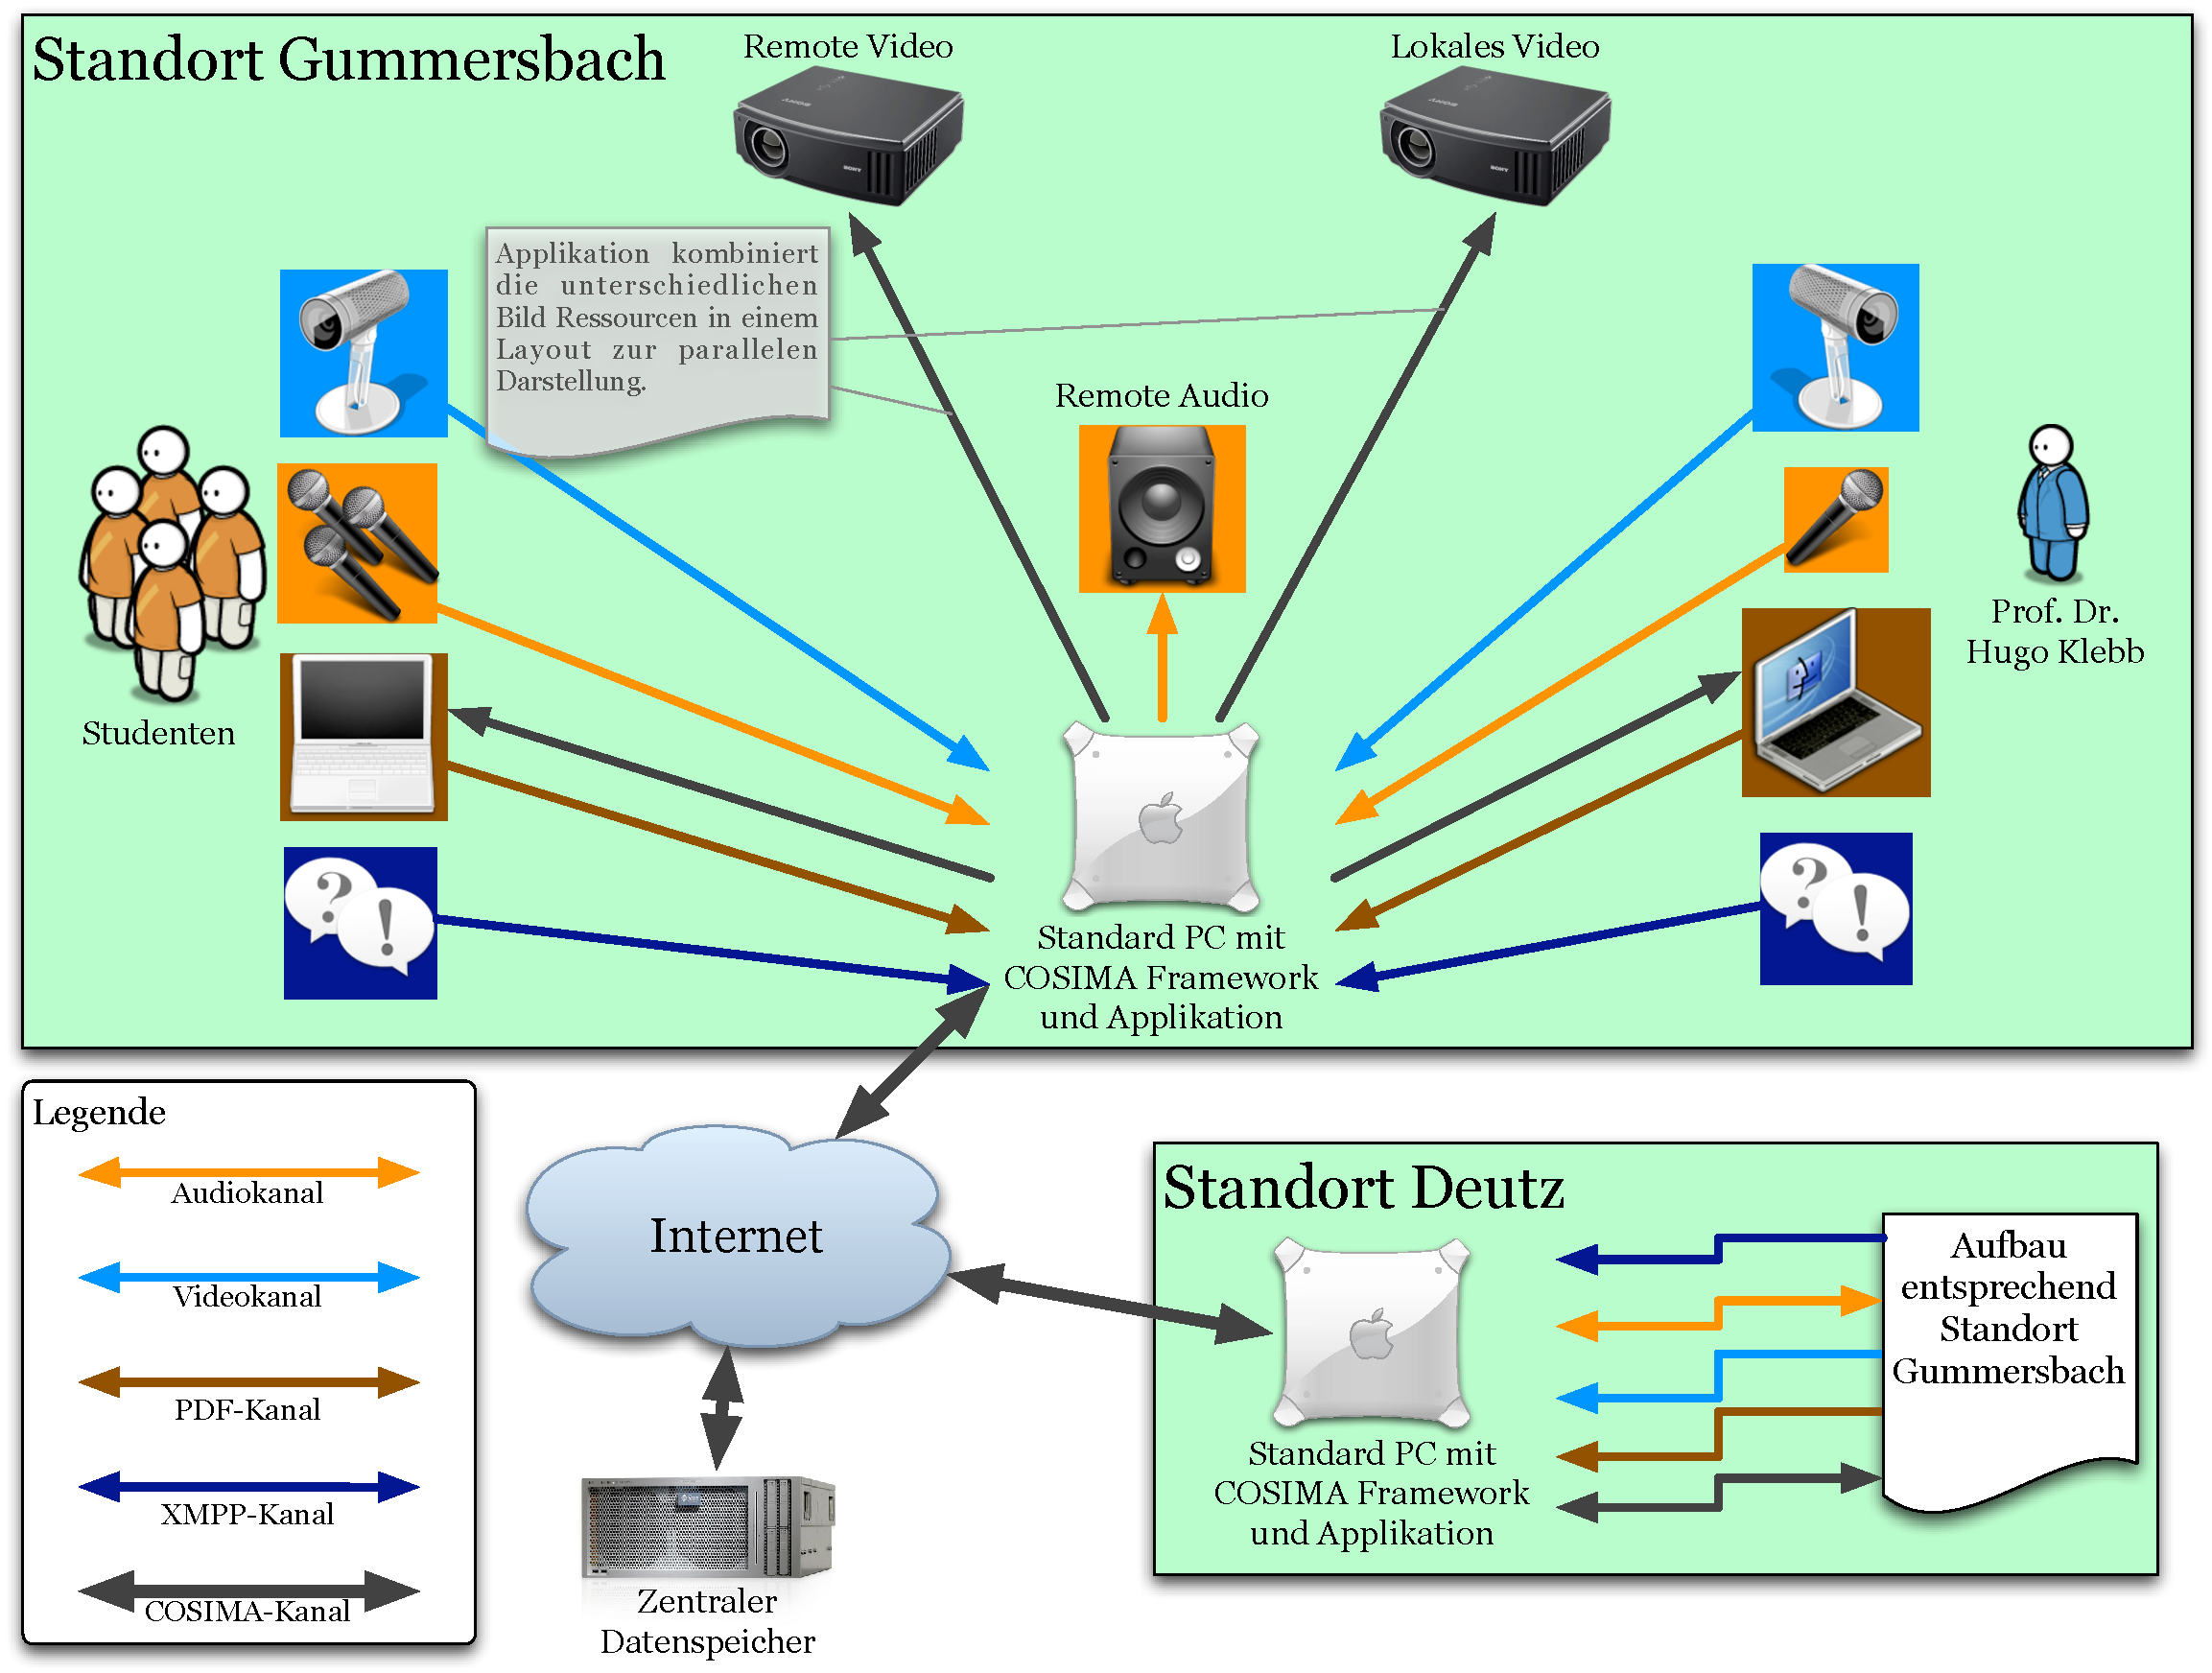
\includegraphics[width=.9\textwidth]{images/Hardware_und_Kanaele.pdf}
    \caption{Schematische Darstellung der Komponenten und ihrer Kommunikationskanäle}
    \label{fig:images_Hardware_und_Kanaele}
  \end{figure}
  
  \begin{itemize}
    \item An jedem Standort sind zwei hochauflösende Kameras installiert. Eine davon filmt den Dozenten, die andere das Auditorium.
    \item An jedem Standort sind zwei Projektoren installiert. Einer zeigt das Videobild der Gegenseite, der andere Folien oder andere Informationen des jeweils nicht-entfernten Standortes.
    \item Jeder Standort verfügt über einen PC, an die alle Ein- und Ausgabegeräte angeschlossen sind, und die Kommunikation zwischen beiden Standorten verwaltet.
    \item Mobile Computersysteme der Studenten oder des Dozenten können bei Bedarf über den Kommunikation-PC in das System integriert werden.
    \item Über ein Dozentenmikrofon sowie Raummikrofone werden die Gespräche erfasst und an die Gegenseite übermittelt.
    \item Jeder Standort verfügt zur Wiedergabe der Audiodaten über ein Lautsprechersystem.
  \end{itemize}
  
\subsection{Zusätzliche Informationen} % (fold)
\label{sub:zusaetzliche_informationen}

  Die Veranstaltung "`Medienrezeption"' findet erfahrungsgemäß im kleinen Kreise statt, da es sich um ein Fach im Masterstudiengang handelt. Etwa 10 Studenten der Medieninformatik besuchen sie. Bei den Medientechnikern wird es nicht als Pflichtfach, sondern als Wahlpflichtfach angeboten, daher nehmen in der Pilotphase nur 5 Studenten aus Deutz teil.

  Es wird für dieses Setup keine außergewöhnliche Technik benötigt, was die Umsetzung deutlich vereinfacht. Bei allen Komponenten handelt es sich um handelsübliche Hardware, wie man sie in jedem Elektronikmarkt erhalten kann. Die gesamte Steuerung und Kommunikation wird durch die Applikation auf den beiden Kommunikationsrechnern geregelt, die dabei auf dem COSIMA-Projekt basiert. Bei den Rechnern handelt es sich ebenfalls um Standard PCs.

  Die Applikation übernimmt unterschiedliche Aufgaben bei diesem Anwendungsfall, so wird von ihr zum einen das Bild beider Kameras übertragen zum anderen auch das Signal der jeweils zusätzlich angeschlossenen Endgeräte, etwa die Laptops der Studenten. Zusätzlich wird das Audiosignal der Mikrofone übertragen. Die Darstellung des Computersignals erfolgt dabei synchron zu der Darstellung des Videosignals. Die Lautstärke der Mikrofone wird von der Applikation automatisch so angepasst, dass der aktuelle Sprecher optimal zu hören ist und nur wenig Umgebungsgeräusche übertragen werden.

  % Was ebenfalls von dem System umgesetzt wird, ist das "`Zeigen"' auf Inhalte, die von den Rechnern der Dozenten oder Studenten kommen. Dies wird einfach dadurch realisiert, dass das komplette Videosignal abgegriffen und übertragen wird. Somit also auch der Mauszeiger. In weiteren Versionen wären hier sicherlich intelligentere Methoden denkbar.

% subsection zusätzliche_informationen (end)

% Weitere Punkte die möglich wären:
% \begin{itemize}
% 
%   \item Hinzufügen der Möglichkeit den Diskurs zu dokumentieren und dann auch mglw. zu persistieren. (Dokumentation/Kommentare via XMPP denkbar?). Nachrichten können dann mit dem Video-/Audiosignal synchronisiert werden.
%   \item Es könnten auch weitere Dokumente live bereitgestellt werden. Oder es kann auf Web-Ressourcen verwiesen werden (am einfachsten auch via XMPP).
%   \item Der Datenkanal der Laptops könnte statt dem VGA-Signal wirklich die Daten transportieren. Statt also ein Videosignal eines PDF-Dokuments zu schicken, könnte das PDF selbst geschickt werden. Eine Beschränkung auf PDF würde im ersten Schritt reichen. Allerdings muss dann auch die Frage gestellt werden in wie weit die Kontrolle über das PDF geregelt wird: Wer darf scrollen? Wer darf kommentieren? Können die Studenten unabhängig scrollen und kommentieren? Werden diese Kommentare dann live wieder bereit gestellt? Wie sieht die Persistierung dieser Kommentare aus?
%   \item Wenn diese reichhaltigen Informationen abgelegt werden, muss es auch eine Möglichkeit geben sie wieder zu finden.
% 
% \end{itemize}

% subsection systemkomponenten (end)

% section hochschulszenario (end)

\section{Das Anwendungsszenario} % (fold)
\label{sub:das_anwendungsszenario}

  Wie bereits zu Beginn dieses Kapitels erwähnt, ist für die Validierung der Architektur im Rahmen dieser Arbeit der Andwendungsentwickler der Stakeholder von Interesse. Es gilt zu validieren, ob sich die Architektur grundsätzlich dazu eignet eine verteilte Multimediaapplikation zu implementieren. Grundlage für die Validierung soll ein \emph{Anwendungsszenario} sein, dass in diesem Abschnitt definiert wird. Die in den vorherigen Abschnitten vorgestellte Situation einer verteilten Lehrveranstaltung bietet den visionären Rahmen für dieses Szenario. Ein Teilbereich der dort beschriebenen Anwendung soll durch den Softwareentwickler implementiert werden.

% section das_anwendungsszenario (end)

% chapter szenario (end)